
\textbf{Stabilty} is a very important notion we would like analyzing of a system in order to study his behaviour over the time.


\section{Some definitions}
Let us  consider the system $\mathcal{S}$ which has state equation equal to $$\dot{x(t)}=f[x(t), u(t),t]$$ with input signal $u(t)$ and \textbf{initial conditions} $x(0)$.\\

\noindent
\textbf{Definition} \textit{(Solution of a system)} The signal resulting from the system integration is a \textbf{function of the time} $x(t), \quad  t\ge0$ which is called the \textbf{solution} of the system {\color{blue}\textbf{corresponding to} the initial state $x(0)$ and the input $u(t)$}.\\

\noindent
\textbf{Definition} \textit{(Trajectory of a system)} The \textbf{set of the points of the state space generated by the solution} is called a \textbf{trajectory of the system} corresponding to the initial state $x(0)$ and the input $u(t)$. \\

\noindent
Let $x(t)$ be the \textit{solution} of the system with the respecto to the couple  (initial condition, input) equal to ($x(0), u(t)$), we call it the \textbf{nominal solution}. If we change a bit the initial state to $x^p(t)\ne x(t)$ but with the same input signal we have the \textbf{perturbed solution}.\\

\begin{figure*}[h]
    \centering
    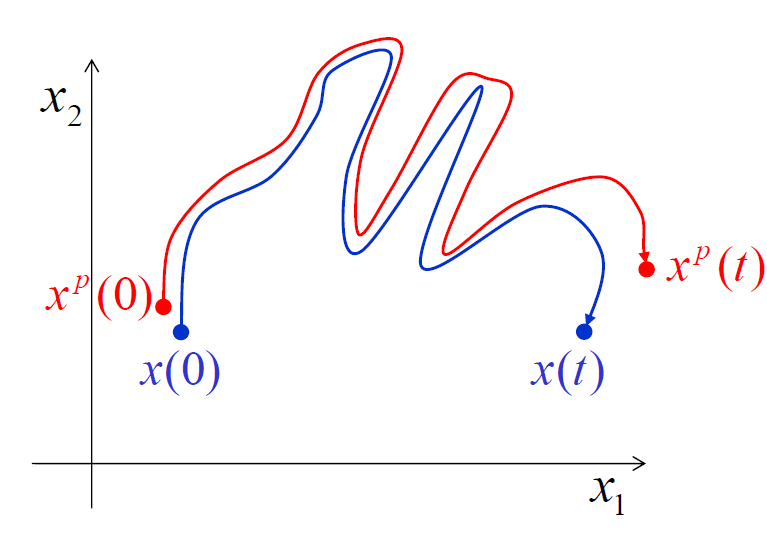
\includegraphics[scale=0.6]{NonLinearControl/images/NominalPerturbed.png}
    \caption{{\color{blue}Nominal solution} and {\color{red}Perturbed solution}} 
    \label{fig:enter-label}
\end{figure*}

\vspace{1cm}
\subsection{Marginal Stability}
\noindent
\textbf{Definition} \textit{(Marginal Stability)} The solution $x(t)$ is \textbf{marginally} (or simply) \textbf{stable} if 
\begin{equation*}
    \forall \epsilon>0, \exists \delta>0 : \\
    \forall x^p(0): \lVert x^p(0)-x(0) \rVert < \delta \Longrightarrow   \lVert x^p(t)-x(t) \rVert < \epsilon, \quad \forall t \ge 0
\end{equation*}
\noindent
{
    \color{blue}
    [Roughly speaking we say that the perturbed solution is always near the nominal solution and so, using other words,  for any choice of $\epsilon$, I am able to find a $\delta$ such that if I choose a perturbed state within the ball of radius $\delta$ for each time $t$, the perturbed solution "fall" within the ball of radius $epsilon$.]
}
\begin{figure}[h]
    \centering
    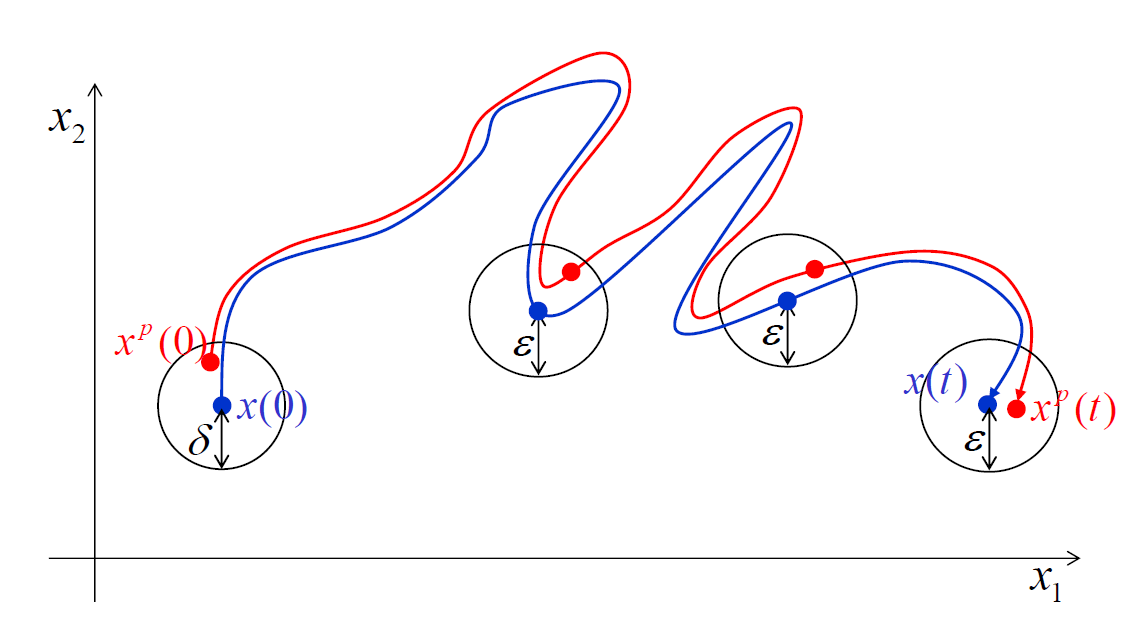
\includegraphics[scale=0.6]{NonLinearControl/images/Stable.png}
    \caption{Marginal stability}
    \label{fig:enter-label}
\end{figure}

\subsection{Asimptotical Stability}
\noindent
\textbf{Definition} \textit{(Asimptotical stability)} The solution $x(t)$ is \textbf{asimptotically stable} if is stable and 
$\lim_{t\to\infty} \lVert x^p(t)-x(t) \rVert=0$. Moreover if the convergence is \textbf{exponential}, the solution is \textbf{exponentially stable}. (This concept is also linked to \textit{modal analysis}.)

\begin{figure}[h]
    \centering
    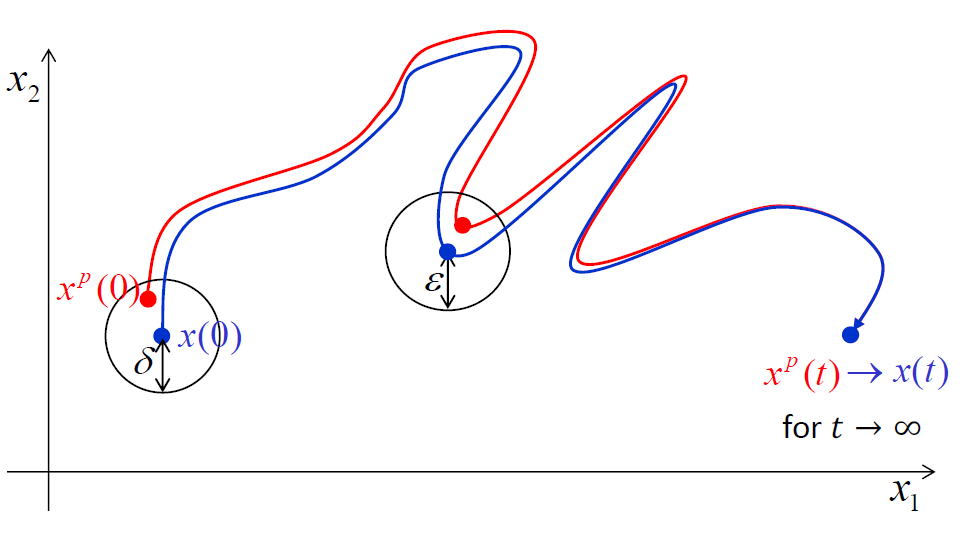
\includegraphics[scale=0.6]{NonLinearControl/images/AsStable.png}
    \caption{Asimptotical stability of a trajectory}
    \label{fig:enter-label}
\end{figure}

\subsection{Unstability}
\noindent
\textbf{Definition} \textit{(Unstability)} A solution of a system is \textbf{unstable} if it is not stable. (Despite I  choose a perturbed initial condition which could be even very close to $x(0)$, the perturbed solution $x^p(t)$ \textbf{go far away} from $x(t)$.

\begin{figure}[h]
    \centering
    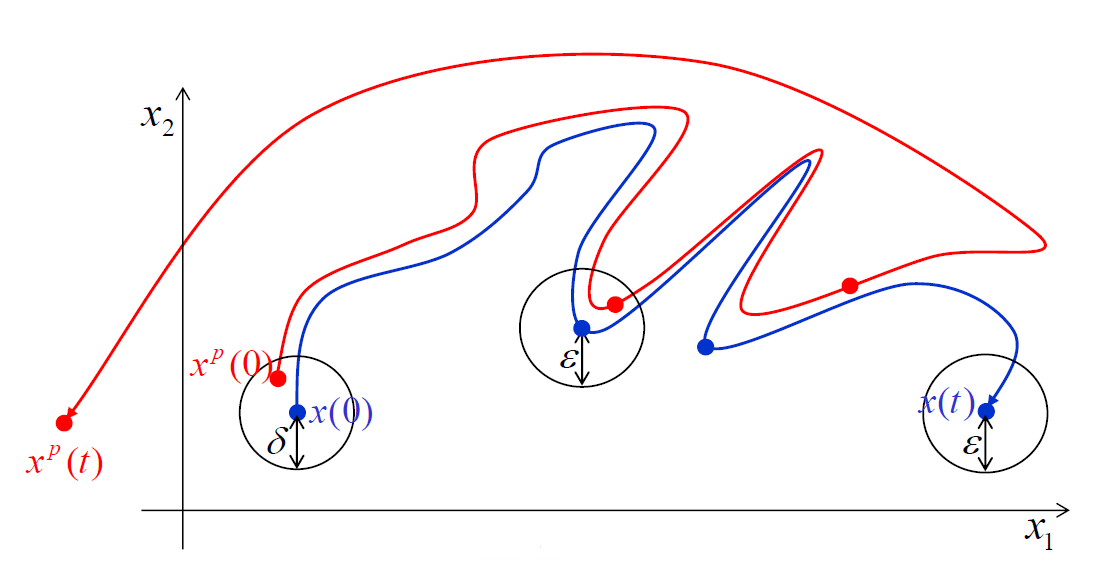
\includegraphics[scale=0.6]{NonLinearControl/images/Unstable.png}
    \caption{Unstable solution}
    \label{fig:enter-label}
\end{figure}

\section{Equilibrium point of a system}

\subsection{Equilibrium point} Given a system with the state equation $\dot{x}=f(\bar{x},\bar{u})$, given a constant input $\bar{u}$, \textbf{$\bar{x}$} is called an \textbf{equilibrium point or state} corresponding to the constant input \textbf{$\bar{u}$}, if it is solution of the equation $$f(\bar{x}, \bar{u})=0$$

\noindent
\textbf{So:} $f(\bar{x}, \bar{u})=0 \Longleftrightarrow \dot{x}=0 \Longleftrightarrow \textrm{null variation over the time} \Longleftrightarrow \textrm{the state remains constant}$

\subsection{Stability of the equilibrium point}

\textbf{Definition} (Stability) The equilibrium point $\bar{x}$ is stable if: 
\begin{equation*}
    \forall \epsilon, \exists \delta: \forall x(0): \lVert x(0)-\bar{x} \rVert \le \delta \Longrightarrow \lVert x(t)-\bar{x} \rVert \le \epsilon, \quad \forall t \ge 0
\end{equation*}
\begin{figure}[h]
    \centering
    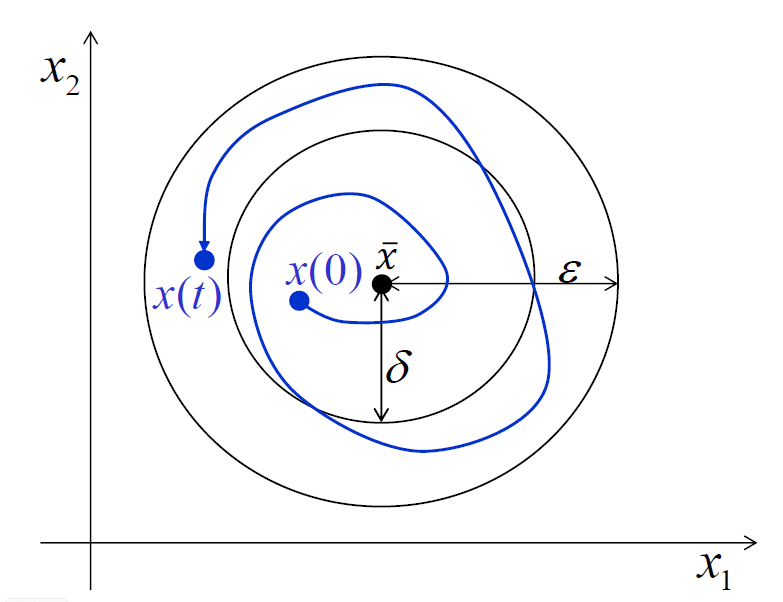
\includegraphics[scale=0.5]{NonLinearControl/images/EqStable.png}
    \caption{Stable equilibrium point}
    \label{fig:enter-label}
\end{figure}

\noindent{
\color{blue}
    A \textbf{simpler explanation} of this concept is that if we move from the equilibrium point choosing a $x(0)$ within a certain ball of radius $\delta$, the equilibrium point itself is stable if the trajectory $x(t)$ remains close to the equilibrium point within another ball of a certain radius $\epsilon$.\\
    
    To find the equilibrium point is sufficient to solve the equation $f(\bar{x}, \bar{u})=0$. Sometimes is quite easy to solve it (e.g. the case of the pendulum), but many times could be not trivial to find an analytical solution.  \\
} 

\noindent
\textbf{Definition} (Asymptotic Stability) The equilibrium state $\bar{x}$ is \textbf{asymptotically stable} if it is stable and it holds that: $$\lim_{t\to \infty} \lVert x(t)-\bar{x} \rVert =0$$

\begin{figure}[h]
    \centering
    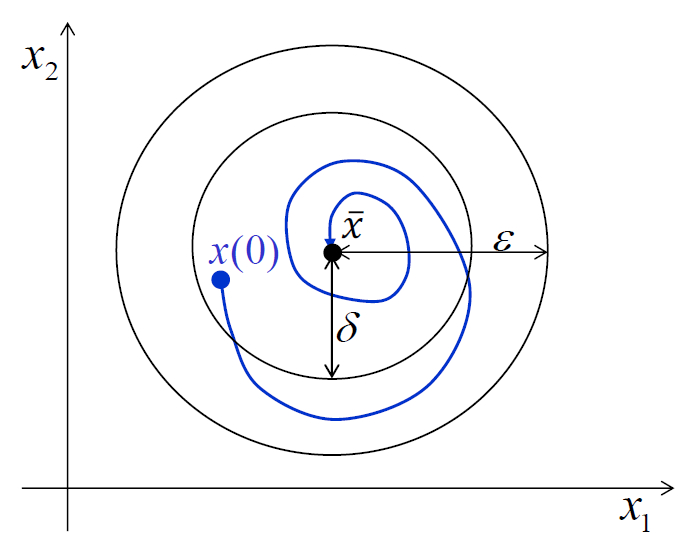
\includegraphics[scale=0.55]{NonLinearControl/images/EqAsStable.png}
    \caption{Asymptotically stable equilibrium point}
    \label{fig:enter-label}
\end{figure}

\noindent
\textbf{Definition} (Instability) The equilibrium state $\bar(x)$ is unstable if it is not stable. That is, Despite we remain close to the equilibrium point the trajectory goes far away the neighbourhood of the point itself.

\begin{figure}[h]
    \centering
    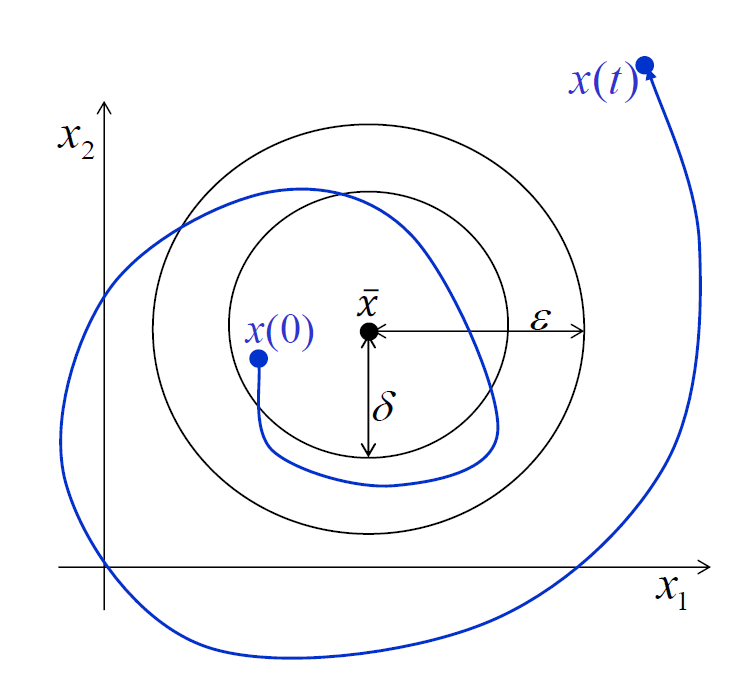
\includegraphics[scale=0.5]{NonLinearControl/images/EqUnstable.png}
    \caption{Unstable equilibrium point}
    \label{fig:enter-label}
\end{figure}

\vspace{1cm}
\noindent
\textbf{Definition} (Domain of attraction) \textbf{A domain of attraction} is a (generic) set of points such that the trajectories initiated at these point converge to the \textit{equilibrium point}. \textbf{The domain of attraction} is the set of \textbf{all points} such that if we start from these point we reach the equilibrium point. If asymptotic stability holds for all initial conditons, then the equilibrium point is \textbf{stable in the large} or \textbf{globally} stable.

\section{Particular case: Stability of LTI systems}
In the case of a Linear Time-Invariant (LTI) system we can write the state solution as $\dot{x}(t)=Ax(t)+Bu(t)$. In this particular case the stability is for the system, not only for a trajectory.\\
For any constant input $\bar{u}$ the equilibrium states can be found \textbf{solving respect to $\bar{x}$} the equation
\begin{equation*}
    \dot{x}=A\bar{x}+B\bar{u}=0 \longleftrightarrow 
    A\bar{x}=-B\bar{u}
\end{equation*}
If $det(A)\ne 0$, then the solution is unique otherwise we can have infinite solutions which generate a subplane (e.g. a line). In the case that $\bar{u}=0$ we obtain a subspace.\\
If $\lambda_1,..., \lambda_i$ are the  \textbf{eigenvalues} of A and $k_1,..., k_i$ are their \textbf{auxiliary geometric multiplicities}, holds that: \\

\noindent
\textbf{Theorem} The LTI system is (internally):
\begin{enumerate}
    \item {\color{red} asymptotically stable} stable if and only if
    $Re(\lambda_i)<0, \forall i$
    \item{\color{red} marginally stable } if and only if $Re(\lambda_i)\le 0, k_i=1 if Re(\lambda_i)=0$
    \item {\color{red} unstable} if and only if
    $\exists i: Re(\lambda_i)>0 \quad \textrm{or} \quad \exists i: Re(\lambda_i)=0, k_i>1$
\end{enumerate}

\noindent
In the case of \textit{non linear systems} the results which has just seen have to be applied to \textbf{each equilibrium point}. It is also of interest to analyze a general property of stability which is the \textbf{BIBO stability} (Bounded Input - Bounded Output), that refers to any type of system of the form 
\begin{align*}
    &\dot{x}=f[x, u, t]\\
    &y=h[x, u, t]
\end{align*}

\noindent
\textbf{Definition} (BIBO stability) A system descripted by the standard state equation  is \textbf{BIBO stable} if \textbf{for any bounded initial condition} and \textbf{for any bounded input} such that $\lVert u(t) \rVert \le M_u < \infty, \forall t \ge 0$ the resulting output is also bounded, that is $\lVert y(t) \rVert \le M_y, \forall t\ge 0$

\noindent
In order to conclude this chapter, we can mention some observation that come from the \textit{modal analysis}: 
\begin{itemize}
    \item asympotic stability $\Longrightarrow$ BIBO stability
    \item BIBO unstability $\Longrightarrow$ instability or marginal stability
\end{itemize}
An example of system that is (simply) stable but NOT BIBO stable is the integrator descripted by the equation
$$\dot{x}(t)=u(t), \quad y(t)=x(t), x,y,u \in \mathbb{R}$$
If we applied a \textbf{constant input} the result \textbf{y(t)} is a ramp. Moreover the BIBO stability is also called \textbf{external stability}.




